\chapter{杂七杂八的话}

\section{Readme}

模板文件的结构, 如下表所示:
 \begin{table}[ht]\centering
\begin{tabular}{r|r|l}
	\hline\hline
	\multicolumn{2}{l|}{main.tex }       & 主文档. 在其中填写正文.             \\ \hline
	                                & frontmatter.tex & 郑重声明、摘要.               \\ \cline{2-3}
	\raisebox{1em}{pages 文件夹} &  backmatter.tex & 实验结论.                       \\ \hline
	\multicolumn{2}{l|}{figures 文件夹}                  & 存放图片文件.                   \\ \hline
	\multicolumn{2}{l|}{WHUBachelor.cls }             & 定义文档格式的 class file. 不可删除. \\ \hline\hline
\end{tabular}
\end{table}

无需也不要改变、移动上述文档的位置.

如果不习惯用~\verb|\include{ }|~的方式加入``子文档'', 当然可以把它们合并在主文档, 成为一个文档.
({\kaishu 但是这样并不会给我们带来方便.})




 \section{字体调节}

\begin{tabular}{ll}
	\verb|\songti|   & {\songti 宋体}   \\
	\verb|\heiti|    & {\heiti 黑体}    \\
	\verb|\fangsong| & {\fangsong 仿宋} \\
	\verb|\kaishu|   & {\kaishu 楷书}
\end{tabular}


\section{字号调节}
字号命令: \verb|\zihao| \index{zihao}

\begin{tabular}{ll}
\verb|\zihao{0}| &\zihao{0}  初号字 English \\
\verb|\zihao{-0}|&\zihao{-0} 小初号 English \\
\verb|\zihao{1} |&\zihao{1}  一号字 English \\
\verb|\zihao{-1}|&\zihao{-1} 小一号 English \\
\verb|\zihao{2} |&\zihao{2}  二号字 English \\
\verb|\zihao{-2}|&\zihao{-2} 小二号 English \\
\verb|\zihao{3} |&\zihao{3}  三号字 English \\
\verb|\zihao{-3}|&\zihao{-3} 小三号 English \\
\verb|\zihao{4} |&\zihao{4}  四号字 English \\
\verb|\zihao{-4}|&\zihao{-4} 小四号 English \\
\verb|\zihao{5} |&\zihao{5}  五号字 English \\
\verb|\zihao{-5}|&\zihao{-5} 小五号 English \\
\verb|\zihao{6} |&\zihao{6}  六号字 English \\
\verb|\zihao{-6}|&\zihao{-6} 小六号 English \\
\verb|\zihao{7} |&\zihao{7}  七号字 English \\
\verb|\zihao{8} |&\zihao{8}  八号字 English \\
\end{tabular}

\section{已加入的常用宏包}

\begin{description}
%  \item[amsmath,amssymb]
  \item[cite]  参考文献引用, 得到形如 [3-7] 的样式.
  \item[color,xcolor]  支持彩色.
  \item[enumerate]  方便自由选择 enumerate 环境的编号方式. 比如

  \verb|\begin{enumerate}[(a)]| 得到形如 (a), (b), (c) 的编号.


  \verb|\begin{enumerate}[i)]| 得到形如 i), ii), iii) 的编号.

  \verb|\begin{enumerate}[\hspace{1cm}(1)]| \verb|\hspace|命令用于调整距离

\end{description}

另外要说明的是,  itemize, enumerate, description 这三种 list 环境, 已经调节了其间距和缩进,
以符合中文书写的习惯.

\section{标点符号的问题}

建议使用半角的标点符号, 后边再键入一个空格. 特别是在英文书写中要注意此问题!

双引号是由两个左单引号、两个右单引号构成的: \verb|``  ''|. 左单引号在键盘上数字~1 的左边.

但是, 无论您偏向于全角或半角, 强烈建议您使用实心的句号, 只要您书写的是自然科学的文章.
原因可能是因为, 比如使用全角句号的句子结尾处的``$x$。''容易误为数学式~$x_0$(\verb|$x_0$|)吧.



\section{引用的问题}


\subsection{参考文献的引用}

参考文献的引用, 用命令~\verb|\cite{ }|. 大括号内要填入的字串, 是自命名的文献条目名.

比如, 通常我们会说:

 {\kaishu
关于此问题, 请参见文献 \cite{r2}. 作者某某还提到了某某概念\upcite{r1}.}


上文使用的源文件为:

 {\kaishu
关于此问题, 请参见文献~\verb|\cite{r2}|. 作者某某还提到了某某概念~\verb|\upcite{r1}|.
}

其中~\verb|\upcite| 是自定义命令, 使文献引用呈现为\CJKunderdot{上标形式}.

({\heiti 注意:} {\kaishu 这里文献的引用, 有时需要以上标形式出现, 有时需要作为正文文字出现, 为什么?})

另外, 要得到形如~\cite{r1,r3,r4,r5} 的参考文献连续引用, 需要用到 cite 宏包(模板已经加入),
在正文中使用~\verb|\cite{r1,r3,r4,r5}| 的引用形式即可.
或者, 连续引用的上标形式: 使用~\verb|\upcite{r1,r2,r3}|, 得到\upcite{r1,r2,r3}.

\subsection{定理和公式的引用}

\begin{theorem}[谁发现的]\label{th-abcd}
最大的正整数是~$1$.
\end{theorem}

\begin{proof}
要找到这个最大的正整数, 我们设最大的正整数为~$x$, 则~$x \geqslant 1$, 两边同时乘以~$x$, 得到
\begin{equation}\label{eq-abc}
x^2 \geqslant x.
\end{equation}
而~$x$ 是最大的正整数, 由~\eqref{eq-abc} 式得到
\[
x^2 = x.
\]
所以
\begin{equation*}
x = 1.
\end{equation*}
\end{proof}

定理~\ref{th-abcd} 是一个重大的发现.

%%%%----- 定义等环境的举例 --------
\begin{definition}[整数]
 正整数(例如 1, 2, 3)、负整数(例如 ${−1}$, $−2$, $−3$)与零(0)合起来统称为{\heiti 整数}.
\end{definition}

\begin{remark}
  整数集合在数学上通常表示为 $\mathbf{Z}$ 或 $\mathbb{Z}$, 该记号源于德语单词 Zahlen(意为``数'')的首字母.
\end{remark}

\begin{proposition}
任意两个整数相加、相减、相乘的结果, 仍然是整数.
\end{proposition}

\begin{example}
  $1+2=3$.
\end{example}

\begin{corollary}
   在整数集合内, 相加、相减、相乘运算是封闭的.
\end{corollary}

\section{图形与表格}

支持对~eps, pdf, jpg 等等常见图形格式.

再次\colorbox{red!45}{澄清一个误会}: \LaTeX{} 支持的图形格式绝非 eps 这一种. 无需特意把图片转化为 eps.

用形如~\verb|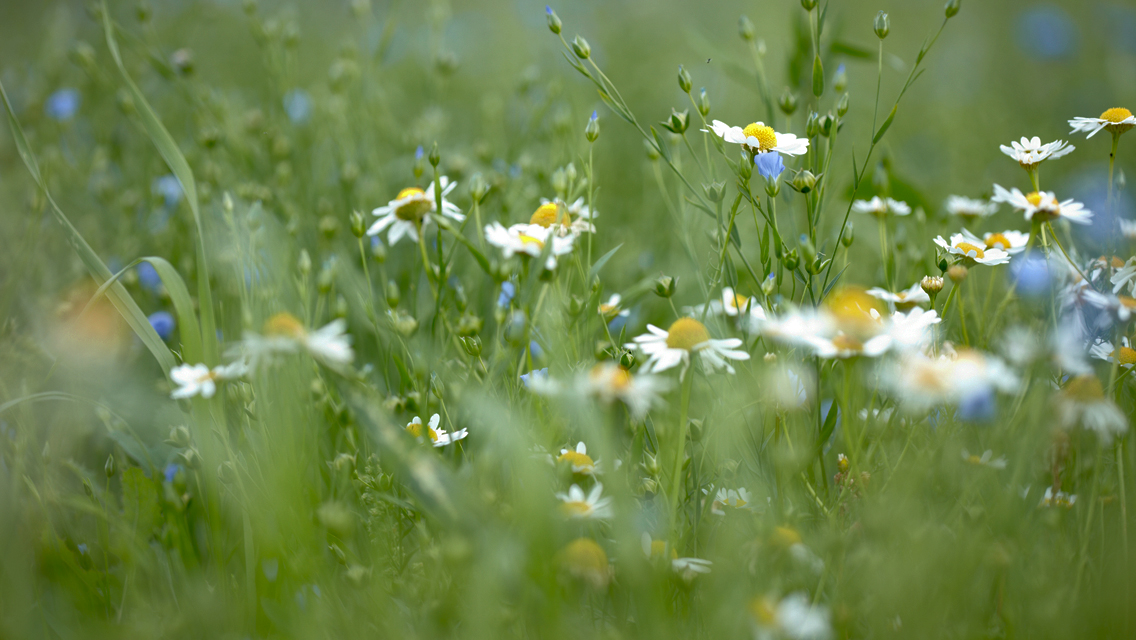
\includegraphics[width=12cm]{Daisy.jpg}| 的命令可以纳入图片.

如图~\ref{fig:1} 是一个纳入~jpg 图片的例子.

\begin{figure}[ht]
\centering
  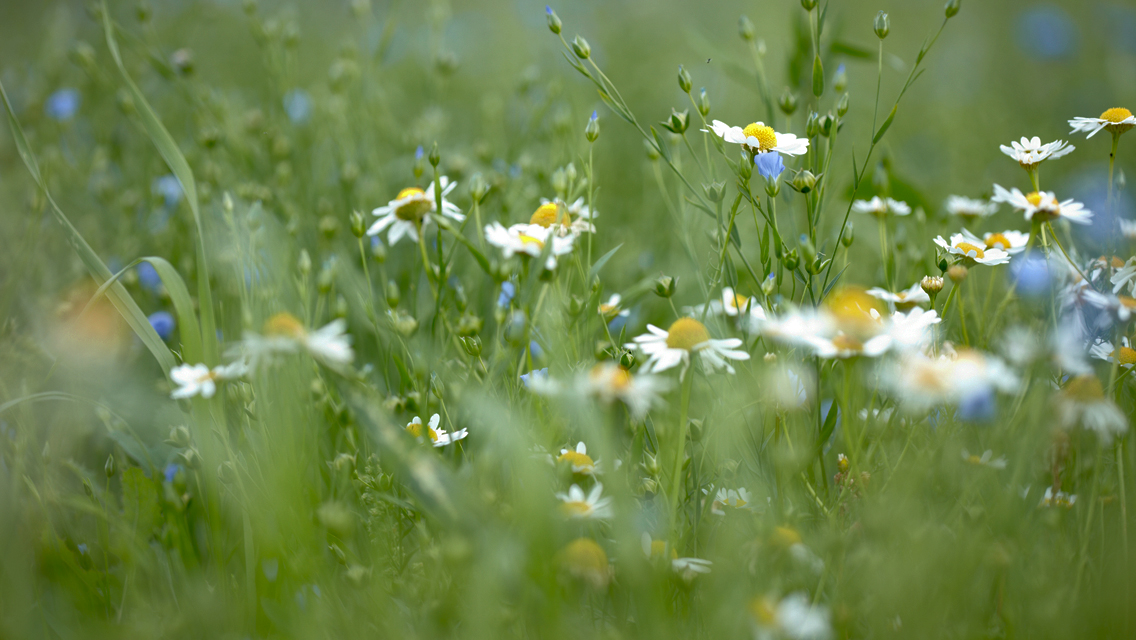
\includegraphics[width=\textwidth]{Daisy.jpg}
  \caption{一个彩色 jpg 图片的例子}
  \label{fig:1}
\end{figure}

表格问题, 建议使用``三线表'', 如表 \ref{tab:1}.

\begin{table}[ht]
\centering
\caption{一般三线表}
\label{tab:1}
    \begin{tabular}{c c c c c c c c c c c}
    \hline
    123 & 4  & 5  & 123 & 4 & 5123 & 4 & 5 & 123 & 4 & 5\\
    \hline
    67 & 890 & 13 & 123 & 4 & 5123 & 4 & 5 & 123 & 4 & 5\\
    67 & 890 & 13 & 123 & 4 & 5123 & 4 & 5 & 123 & 4 & 5\\
    67 & 890 & 13 & 123 & 4 & 5123 & 4 & 5 & 123 & 4 & 5\\
    \hline
    \end{tabular}
\end{table}
